\section{Modellierung der Systemdynamik} \label{Dynamik_sec}
In dem folgenden Abschnitt werden die Bewegungsgleichungen mit Hilfe des Lagrange Formalismus hergeleitet. Aus diesen Gleichung kann im Anschluss eine Zustandsraumdarstellung aufgestellt werden, welche als Grundlage für den Reglerentwurf dient.

\begin{figure}[h]
\centering
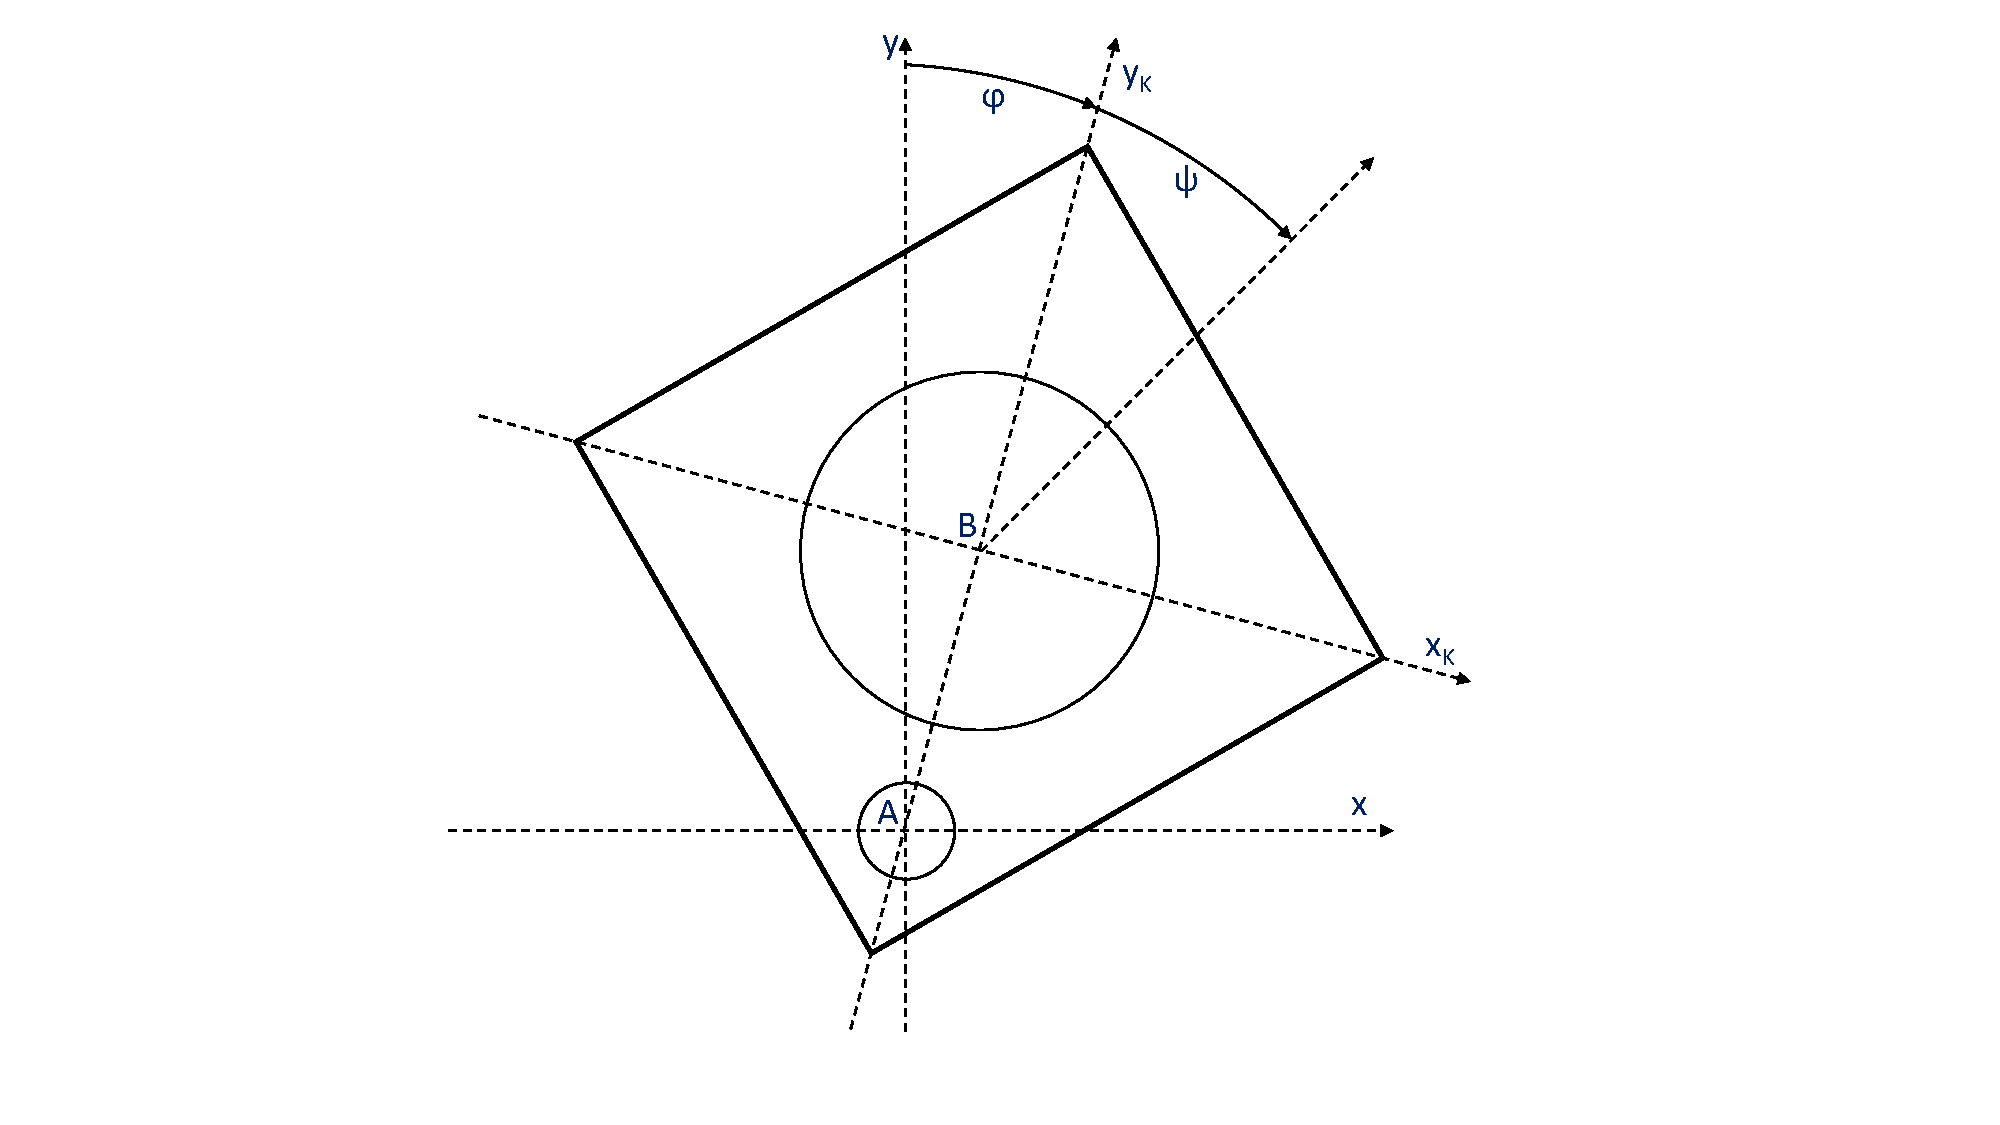
\includegraphics[width=\linewidth]{MechZeichnung1D}
\caption{Mechanischer Aufbau, Quelle: eigene Darstellung}
\end{figure}

Der Prototyp besteht aus einem starren Körper der in $A$ auf einer Achse gelagert ist. In $B$ ist eine Schwungmasse über einen Motor mit dem Körper verbunden. Somit verfügt das Gesamtsystem über zwei Freiheitsgrade, welche durch die generalisierten Koordinaten 

\begin{equation}
q_1 = \varphi \hspace{35pt} q_2 = \psi
\end{equation}

beschrieben werden. Der Winkel $\varphi$ wird von den Achsen $y$ und $y_K$ eingeschlossen. Der Winkel beschreibt die rotatorische Verschiebung der Schwungmasse zu dem Körper. Die folgenden Größen beschreiben die weiteren physikalischen Gegebenheiten des Systems.\newline

\begin{table}[h]
\centering
\begin{tabular}{ll}
	$q_1 = \varphi$ & Ausfallwinkel des Körpers \\
	$q_2 = \psi$ & Winkel zwischen Schwungmasse und Körper \\
	$A$ & Drehpunkt des Körpers \\
	$B$ & Drehpunkt des Schwungrades \\
	$l_{AB}$ & Abstand zwischen $A$ und $B$ \\
	$l_{AC}$ & Abstand zwischen $A$ und dem Schwerpunkt des Körpers \\
	$m_K$ & Masse des Körpers \\
	$m_R$ & Masse des Schwungrades \\
	${\theta}^A_K$ & Massenträgheitsmoment des Körper um $A$ \\
	${\theta}^B_R$ & Massenträgheitsmoment der Schwungmasse um $B$ \\
	$C_{\varphi}$ & Dynamischer Reibkoeffizient des Körpers in $A$ \\
	$C_{\psi}$ & Dynamischer Reibkoeffizient des Schwungrades in $B$ \\
	$T_M$ & Drehmoment des Motor
\end{tabular}
\end{table}

\newpage
Um die Bewegungsgleichungen des Systems zu ermitteln wird der Lagrange Formalismus verwendet. Dieser basiert auf der Lagrange-Funktion $L$, welche die Differenz der kinetischen Energie $T$ und der potenziellen Energie $V$ des Systems beschreibt.

\begin{equation}
T = \frac{1}{2}[({\theta}^A_K + m_R \cdot {l_{AB}}^2) {\dot{\varphi}}^2 + {\theta}^R_B(\dot{\varphi}+\dot{\psi})^2]
\end{equation}
\begin{equation}
V = g(m_R \cdot l_{AB} + m_K \cdot l_{AC})cos(\varphi)
\end{equation}
\begin{equation}
L = T - V = \frac{1}{2}[({\theta}^A_K + m_R \cdot {l_{AB}}^2) {\dot{\varphi}}^2 + {\theta}^R_B(\dot{\varphi}+\dot{\psi})^2] - g(m_R \cdot l_{AB} + m_K \cdot l_{AC})cos(\varphi)
\end{equation}

In dem System wirken unterschiedliche Kräfte. Einerseits erzeugt der Motor ein Drehmoment, welches die virtuelle Arbeite $\delta W_M$ verursacht. Andererseits verrichtet die Gravitation die virtuelle Arbeite $\delta W_G$. Zusätzlich muss die, durch die Reibung entstandene, Verlustleistung berücksichtigt werden. In diesem Fall wird die Reibleistung mit den Rayleigh'schen Dissipationsfunktionen $D_{\varphi}$ und $D_{\psi}$ beschrieben und verrichten die virtuelle Arbeit $\delta W_D$.

\begin{equation}
-\delta W_M = T_M \cdot \delta \psi
\end{equation}

\begin{equation}
-\delta W_G = g(m_K \cdot l_{AC} + m_R \cdot l_{AB})sin(\varphi) \cdot \delta \varphi
\end{equation}

\begin{equation}
D_{\varphi} = \frac{1}{2}C_{\varphi} \cdot {\dot{\varphi}}^2
\end{equation}
\begin{equation}
D_{\psi} = \frac{1}{2}C_{\psi} \cdot {\dot{\psi}}^2
\end{equation}
\begin{equation}
D = D_{\varphi} + D_{\psi} = \frac{1}{2}C_{\varphi} \cdot {\dot{\varphi}}^2 + \frac{1}{2}C_{\psi} \cdot {\dot{\psi}}^2
\end{equation}
\begin{equation}
-\delta W_D = - C_{\varphi} \cdot \dot{\varphi} \cdot \delta \varphi - C_{\psi} \cdot \dot{\psi} \cdot \delta \psi
\end{equation}

Die Summe der virtuellen Arbeiten, welche von den verschiedenen Kräften verrichtet wird, ergibt die virtuelle Arbeit des Gesamtsystems $\delta W$. In dem die verrichtete Arbeit partiell nach den beiden generalisierten Koordinaten $\varphi$ und $\psi$ differenziert wird, können die beiden generalisierten Kraftkomponenten $Q_{\varphi}$ und $Q_{\psi}$ berechnet werden.

\begin{equation}
Q_{\varphi} = g(m_K \cdot l_{AC} + m_R \cdot l_{AB})sin(\varphi) - C_{\varphi} \cdot \dot{\varphi}
\end{equation}
\begin{equation}
Q_{\psi} = T_M - C_{\psi} \cdot \dot{\psi}
\end{equation}


Bei dem Prototyp handelt es sich um ein nicht konservatives System, da durch die Reibung mechanische Energie verloren geht und der Motor dem System mechanische Energie zuführt. Da die beiden generalisierten Koordinaten $\varphi$ und $\psi$ voneinander unabhängig sind können aus dem d'Alembert'schen Prinzip zwei Bewegungsgleichungen abgeleitet werden.

\begin{equation}
\frac{d}{dt}\frac{\partial T}{\partial \dot{q}_i}-\frac{\partial T}{\partial q_i} = Q_i
\end{equation}
\begin{equation}
\frac{d}{dt}\frac{\partial T}{\partial \dot{\varphi}}-\frac{\partial T}{\partial \varphi} = Q_{\varphi} 
\end{equation}
\begin{equation}
\label{LG_phi_equation}
({\theta}^A_K + {\theta}^B_R + m_R \cdot l_{AB}^2)\ddot{\varphi} + {\theta}^B_R \cdot \ddot{\psi} - g(m_R \cdot l_{AB} + m_K \cdot l_{AC})sin(\varphi) + C_{\psi} \cdot \dot{\psi} = 0
\end{equation}
\begin{equation}
\frac{d}{dt}\frac{\partial T}{\partial \dot{\psi}}-\frac{\partial T}{\partial \psi} + \frac{\partial T}{\partial \dot{\psi}} = Q_{\psi} 
\end{equation}
\begin{equation}
\label{LG_psi_euqation}
{\theta}^R_B \cdot \ddot{\psi} = T_M - C_{\psi} \cdot \dot{\psi} - {\theta}^B_R \cdot \ddot{\varphi}
\end{equation}

Durch Einsetzen von (\ref{LG_psi_euqation}) in (\ref{LG_phi_equation}) ergibt sich die folgende Bewegungsgleichung für die Würfelseite.

\begin{equation}
\label{BG_phi_quation}
\ddot{\varphi} = \frac{g(m_R \cdot l_{AB}^2 + m_K \cdot l_{AC})sin(\varphi) - C_{\varphi} \cdot \dot{\varphi} + C_{\psi} \cdot \dot{\psi} - T_M}{{\theta}^A_K + m_R \cdot l_{AB}^2}
\end{equation}

Die Bewegungsgleichung für die Schwungmasse ergibt sich durch Einsetzen von (\ref{BG_phi_quation}) in (\ref{LG_psi_euqation}).

\begin{equation}
\label{BG_psi_equation}
\ddot{\psi} = \frac{({\theta}^A_K + m_R \cdot l_{AB}^2 + {\theta}^B_R)(T_M - C_{\psi} \cdot \dot{\psi})}{({\theta}^A_K + m_R \cdot {l_{AB}}^2){\theta}^B_R} + \frac{C_{\varphi} \cdot \dot{\varphi} - g(m_R \cdot l_{AB} + m_K \cdot l_{AC})sin(\varphi)}{{\theta}^A_K + m_R \cdot {l_{AB}}^2}
\end{equation}